\subsection{Results on Empirical Data}

\begin{figure}[htbp]
    \centering
    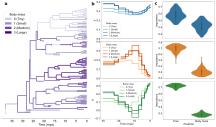
\includegraphics[width=1\textwidth]{figures/platyrrhine.pdf}
    \caption{Results for the Platyrrhine empirical dataset. The panels display, from left to right, the median estimates across all replicate trees for (a) the speciation rate (\( \lambda \)); (b) the extinction rate (\( \mu \)); and (c) the diversification rate (\( d = \lambda - \mu \)).}%
    \label{fig:platyrrhine}
\end{figure}

\begin{figure}[htbp]
    \centering
    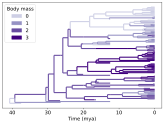
\includegraphics[width=1\textwidth]{figures/platyrrhine-type-tree.pdf}
    \caption{Estimated body masses for each branch in a representative Platyrrhine tree, computed as the median estimated body mass per branch.}%
    \label{fig:platyrrhine-type-tree}
\end{figure}

\begin{figure}[htbp]
    \centering
    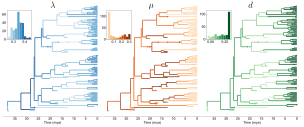
\includegraphics[width=1\textwidth]{figures/platyrrhine-trees.pdf}
    \caption{Median estimates for each branch for a representative Platyrrhine tree, showing (a) the speciation rate (\( \lambda \)); (b) the extinction rate (\( \mu \)); and (c) the diversification rate (\( d = \lambda - \mu \)). Each panel includes an inset histogram illustrating the distribution of the corresponding rate across the tree.}%
    \label{fig:platyrrhine-trees}
\end{figure}

\begin{figure}[htbp]
    \centering
    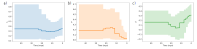
\includegraphics[width=1\textwidth]{figures/platyrrhine-marginal.pdf}
    \caption{Marginal estimates and 95\% credible intervals for (a) the speciation rate (\( \lambda \)); (b) the extinction rate (\( \mu \)); and (c) the diversification rate (\( d = \lambda - \mu \)) for a representative Platyrrhine tree.}%
    \label{fig:platyrrhine-marginal}
\end{figure}

Figure~\ref{fig:platyrrhine} summarizes the results obtained by applying our Bayesian MLP model to the empirical dataset of Platyrrhine primates. The analysis aimed to estimate the speciation rate (\( \lambda \)), extinction rate (\( \mu \)), and diversification rate (\( d = \lambda - \mu \)) over time, across groups of species classified by a four-level trait representing body mass (0: small, 1: medium-small, 2: medium-large, 3: large). Both time and body mass were included as predictors of the evolutionary rates.

For a representative replicate tree, the estimated body masses for each branch are shown in Figure~\ref{fig:platyrrhine-type-tree}, while Figure~\ref{fig:platyrrhine-trees} displays the median branch-specific estimates of the evolutionary rates, and Figure~\ref{fig:platyrrhine-marginal} presents the marginal estimates with their associated uncertainty intervals.

Overall, the model captures a mixed influence of time and body mass on the evolutionary dynamics. The speciation rate (\( \lambda \)) remains relatively constant across both predictors, showing only minor temporal fluctuations and limited dependence on body mass. In contrast, the extinction rate (\( \mu \)) exhibits a stronger interaction between time and body mass: larger-bodied species experience a pronounced spike in extinction around 10 million years ago, followed by a rapid decline toward the present, whereas smaller-bodied species show a more gradual and later decrease. Consequently, the diversification rate (\( d \)) also reflects this interaction---larger-bodied species undergo a temporary reduction in diversification around 10 million years ago, while smaller-bodied species maintain a relatively stable rate. After this period, all body mass groups exhibit an upward trend in diversification approaching the present.
